\let\negmedspace\undefined
\let\negthickspace\undefined
\documentclass[journal]{IEEEtran}
\usepackage[a5paper, margin=10mm, onecolumn]{geometry}
\usepackage{lmodern}
\usepackage{tfrupee}
\setlength{\headheight}{1cm}
\setlength{\headsep}{0mm}
\usepackage{gvv-book}
\usepackage{gvv}
\usepackage{cite}
\usepackage{amsmath,amssymb,amsfonts,amsthm}
\usepackage{algorithmic}
\usepackage{graphicx}
\usepackage{textcomp}
\usepackage{xcolor}
\usepackage{txfonts}
\usepackage{listings}
\usepackage{enumitem}
\usepackage{mathtools}
\usepackage{gensymb}
\usepackage{comment}
\usepackage[breaklinks=true]{hyperref}
\usepackage{tkz-euclide}
\usepackage{listings}
\usepackage{color}
\usepackage{array}
\usepackage{longtable}
\usepackage{calc}
\usepackage{multirow}
\usepackage{hhline}
\usepackage{ifthen}
\usepackage{lscape}
\usepackage{multicol}


% Footer macro
\newcommand{\qfooter}{%
  \begin{flushright}\footnotesize\textbf{[GATE EE 2025]}\end{flushright}\vspace{1em}%
}

\begin{document}
\bibliographystyle{IEEEtran}
\vspace{3cm}
\title{DA24S1 - Data Science and Artificial Intelligence}
\author{EE25BTECH11009 - ANSHU KUMAR RAM}
{\let\newpage\relax\maketitle}


\begin{enumerate}
%---Q1---%
\item If ‘$\rightarrow$’ denotes increasing order of intensity, then the meaning of the words $[$sick $\rightarrow$ infirm $\rightarrow$ moribund$]$ is analogous to $[$silly $\rightarrow$ \rule{6em}{0.05em} $\rightarrow$ daft$]$.
Which one of the given options is appropriate to fill the blank?
\begin{multicols}{2}
\begin{enumerate}
\item frown
\item fawn
\item vein
\item vain
\end{enumerate}
\qfooter
\end{multicols}

%---Q2---%
\item The 15 parts of the given figure are to be painted such that no two adjacent parts with shared boundaries (excluding corners) have the same color. The minimum number of colors required is:
\begin{multicols}{2}
\begin{enumerate}
\item 4
\item 3
\item 5
\item 6
\end{enumerate}
\qfooter
\end{multicols}

%---Q3---%
\item How many 4-digit positive integers divisible by 3 can be formed using only the digits $\{1,3,4,6,7\}$, such that no digit appears more than once in a number?
\begin{multicols}{2}
\begin{enumerate}
\item 24
\item 48
\item 72
\item 12
\end{enumerate}
\qfooter
\end{multicols}

%---Q4---%
\item The sum of the following infinite series is:
\begin{align}
2 + \frac{1}{2} + \frac{1}{3} + \frac{1}{4} + \frac{1}{8} + \frac{1}{9} + \frac{1}{16} + \frac{1}{27} + \cdots
\end{align}
\begin{multicols}{2}
\begin{enumerate}
\item $\frac{11}{3}$
\item $\frac{7}{2}$
\item $\frac{13}{4}$
\item $\frac{9}{2}$
\end{enumerate}
\qfooter
\end{multicols}

% Q5
\item In an election, the share of valid votes received by the four candidates A, B, C, and D is represented by the pie chart shown.  
The total number of votes cast in the election were 115{,}000, out of which 5{,}000 were invalid.
\begin{figure}[h]
    \centering
    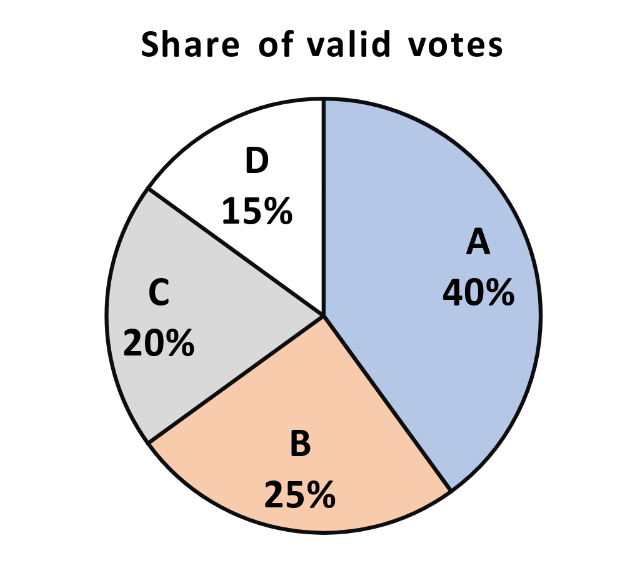
\includegraphics[width=0.45\columnwidth]{figs/q5.png}
    \caption{Share of valid votes}
\label{fig:q5} 
\end{figure}
Based on the data provided, the total number of valid votes received by the candidates B and C is:
\begin{enumerate}
\begin{multicols}{4}
\item 45{,}000
\item 49{,}500
\item 51{,}750
\item 54{,}000
\end{multicols}
\qfooter
\end{enumerate}

% Q6
\item Thousands of years ago, some people began dairy farming. This coincided with a  
number of mutations in a particular gene that resulted in these people developing the ability to digest dairy milk.  
Based on the given passage, which of the following can be inferred?
\begin{enumerate}
\item All human beings can digest dairy milk.
\item No human being can digest dairy milk.
\item Digestion of dairy milk is essential for human beings.
\item In human beings, digestion of dairy milk resulted from a mutated gene.
\qfooter
\end{enumerate}
%---Q7---%
\item The probability of a boy or a girl being born is $\frac{1}{2}$. For a family having only three children, what is the probability of having two girls and one boy?
\begin{multicols}{4}
\begin{enumerate}
\item $\frac{3}{8}$
\item $\frac{1}{8}$
\item $\frac{1}{4}$
\item $\frac{1}{2}$
\end{enumerate} 
\qfooter
\end{multicols}

% Q8
\item Person 1 and Person 2 invest in three mutual funds A, B, and C. The amounts they invest in each are:
\begin{center}
\begin{tabular}{ll}
    \textbf{Group I} & \textbf{Group II} \\
    P. Ferrite & 1. Hexagonal Close Packed (HCP) \\
    Q. Austenite & 2. Body Centered Cubic (BCC) \\
    R. Martensite & 3. Body Centered Tetragonal (BCT) \\
    & 4. Face Centered Cubic (FCC)
\end{tabular}
\end{center}
At the end of one year, Person 1 gets Rs. 500 more than Person 2. Funds B and C earn 15\% annual return.  
What is the annual rate of return for fund A?
\begin{enumerate}
\begin{multicols}{4}
\item 7.5\%
\item 10\%
\item 15\%
\item 20\%
\end{multicols}
\qfooter
\end{enumerate}
 
%---Q9---%
\item Three different views of a dice are shown in the figure below.

\begin{figure}[h]
\centering
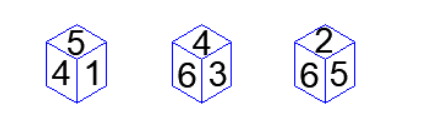
\includegraphics[width=0.42\columnwidth]{figs/q9.png} % <-- insert correct folder and filename
\caption*{Views of the dice}
\label{fig:q9}
\end{figure}

The piece of paper that can be folded to make this dice is

\begin{enumerate}
\item  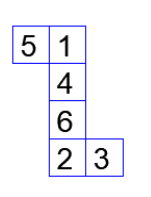
\includegraphics[width=0.17\columnwidth]{figs/q9a.png}
\item  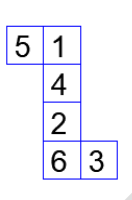
\includegraphics[width=0.17\columnwidth]{figs/q9b.png}
\item  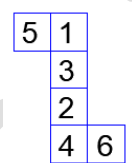
\includegraphics[width=0.17\columnwidth]{figs/q9c.png}
\item  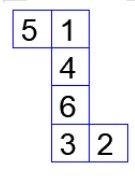
\includegraphics[width=0.17\columnwidth]{figs/q9d.png}
\qfooter
\end{enumerate} 

%---Q10---%
\item Visualize two identical right circular cones such that one is inverted over the other and they share a common circular base. If a cutting plane passes through the vertices of the assembled cones, what shape does the outer boundary of the resulting cross-section make?
\begin{multicols}{2}
\begin{enumerate}
\item A rhombus
\item A triangle
\item An ellipse
\item A hexagon
\end{enumerate}
\qfooter
\end{multicols}

\item Consider the following statements:
\begin{itemize}[leftmargin=*]
    \item[(i)] The mean and variance of a Poisson random variable are equal.
    \item[(ii)] For a standard normal random variable, the mean is zero and the variance is one.
\end{itemize}
Which ONE of the following options is correct?
\begin{multicols}{2}
\begin{enumerate}
\item Both (i) and (ii) are true
\item (i) is true and (ii) is false
\item (ii) is true and (i) is false
\item Both (i) and (ii) are false
\end{enumerate} \qfooter
\end{multicols}

\item Three fair coins are tossed independently. $T$ is the event that two or more tosses result in heads. $S$ is the event that two or more tosses result in tails. What is the probability of the event $T \cap S$?
\begin{multicols}{4}
\begin{enumerate}
\item 0
\item 0.5
\item 0.25
\item 1
\end{enumerate} 
\qfooter
\end{multicols}

\item Consider the matrix $\mtx{M} = \begin{pmatrix}2 & -1\\3 & 1\end{pmatrix}$. Which ONE of the following statements is TRUE?

\begin{enumerate}
\item The eigenvalues of $\mtx{M}$ are non-negative and real.
\item The eigenvalues of $\mtx{M}$ are complex conjugate pairs.
\item One eigenvalue of $\mtx{M}$ is positive and real, and another eigenvalue of $\mtx{M}$ is zero.
\item One eigenvalue of $\mtx{M}$ is non-negative and real, and another eigenvalue of $\mtx{M}$ is negative and real.
\end{enumerate} 
\qfooter


\item Consider performing depth-first search (DFS) on an undirected and unweighted graph $G$ starting at vertex $s$. For any vertex $u$ in $G$, $d[u]$ is the length of the shortest path from $s$ to $u$. Let $(u, v)$ be an edge in $G$ such that $d[u] < d[v]$. If the edge $(u, v)$ is explored first in the direction from $u$ to $v$ during the above DFS, then $(u, v)$ becomes a \rule{7em}{0.07em} edge.
\begin{multicols}{4}
\begin{enumerate}
\item tree
\item cross
\item back
\item gray
\end{enumerate}
\qfooter
\end{multicols}

\item For any twice differentiable function $f: \mathbb{R} \rightarrow \mathbb{R}$, if at some $x^*\in \mathbb{R}$, $f'(x^*)=0$ and $f''(x^*)>0$, then the function $f$ necessarily has a \rule{7em}{0.07em} at $x = x^*$.\\
Note: $\mathbb{R}$ denotes the set of real numbers.
\begin{multicols}{2}
\begin{enumerate}
\item local minimum
\item global minimum
\item local maximum
\item global maximum
\end{enumerate} \qfooter
\end{multicols}

\item Match the items in Column 1 with the items in Column 2 in the following table:
\begin{center}
\begin{tabular}{ll}
Column 1 & Column 2 \\
(p) First In First Out & (i) Stacks \\
(q) Lookup Operation & (ii) Queues \\
(r) Last In First Out & (iii) Hash Tables \\
\end{tabular}
\end{center}
\begin{multicols}{2}
\begin{enumerate}
\item (p)-(ii), (q)-(iii), (r)-(i)
\item (p)-(ii), (q)-(i), (r)-(iii)
\item (p)-(i), (q)-(ii), (r)-(iii)
\item (p)-(i), (q)-(iii), (r)-(ii)
\end{enumerate} \qfooter
\end{multicols}

\item Consider the dataset with six datapoints $\{(\vec{x}_1, y_1), (\vec{x}_2, y_2), \ldots, (\vec{x}_6, y_6)\}$, where\\
$\vec{x}_1 = \myvec{1\\0}$,\quad $\vec{x}_2 = \myvec{0\\1}$,\quad $\vec{x}_3 = \myvec{0\\-1}$,\quad $\vec{x}_4 = \myvec{-1\\0}$,\quad $\vec{x}_5 = \myvec{2\\2}$,\quad $\vec{x}_6 = \myvec{-2\\-2}$,\\
and the labels are $y_1 = y_2 = y_5 = 1$ and $y_3 = y_4 = y_6 = -1$. A hard margin linear support vector machine is trained on the above dataset. Which ONE of the following sets is a possible set of support vectors?
\begin{multicols}{2}
\begin{enumerate}
\item $\{\vec{x}_1, \vec{x}_2, \vec{x}_5\}$
\item $\{\vec{x}_3, \vec{x}_4, \vec{x}_5\}$
\item $\{\vec{x}_4, \vec{x}_5\}$
\item $\{\vec{x}_1, \vec{x}_2, \vec{x}_3, \vec{x}_4\}$
\end{enumerate} \qfooter
\end{multicols}

\item Match the items in Column 1 with the items in Column 2 in the following table:
\begin{center}
\begin{tabular}{ll}
Column 1 & Column 2 \\
(p) Principal Component Analysis & (i) Discriminative Model\\
(q) Na\"ive Bayes Classification & (ii) Dimensionality Reduction\\
(r) Logistic Regression& (iii) Generative Model\\
\end{tabular}
\end{center}
\begin{multicols}{2}
\begin{enumerate}
\item (p)-(iii), (q)-(i), (r)-(ii)
\item (p)-(ii), (q)-(i), (r)-(iii)
\item (p)-(ii), (q)-(iii), (r)-(i)
\item (p)-(iii), (q)-(ii), (r)-(i)
\end{enumerate}
\qfooter
\end{multicols}

\item Euclidean distance based $k$-means clustering algorithm was run on a dataset of $100$ points with $k=3$. If the points $\myvec{1\\1}$ and $\myvec{-1\\1}$ are both part of cluster 3, then which ONE of the following points is necessarily also part of cluster 3?
\begin{multicols}{4}
\begin{enumerate}
\item $\myvec{0\\0}$
\item $\myvec{0\\2}$
\item $\myvec{2\\0}$
\item $\myvec{0\\1}$
\end{enumerate} 
\qfooter
\end{multicols}

\item Given a dataset with $K$ binary-valued attributes (where $K > 2$) for a two-class classification task, the number of parameters to be estimated for learning a na\"ive Bayes classifier is
\begin{multicols}{2}
\begin{enumerate}
\item $2K+1$
\item $2K+1$
\item $2K+1+1$
\item $K^2+1$
\end{enumerate} \qfooter
\end{multicols}


\item Consider performing uniform hashing on an open address hash table with load factor $\alpha = \frac{n}{m} < 1$, where $n$ elements are stored in the table with $m$ slots. The expected number of probes in an unsuccessful search is at most $\frac{1}{1-\alpha}$. Inserting an element in this hash table requires at most \rule{8em}{0.07em} probes, on average.
\begin{multicols}{2}
\begin{enumerate}
\item $\ln\left(\frac{1}{1-\alpha}\right)$
\item $\frac{1}{1-\alpha}$
\item $1+\frac{\alpha}{2}$
\item $\frac{1}{1+\alpha}$
\end{enumerate} \qfooter
\end{multicols}

\item For any binary classification dataset, let $S_B \in \mathbb{R}^{d \times d}$ and $S_W \in \mathbb{R}^{d \times d}$ be the between-class and within-class scatter (covariance) matrices, respectively. The Fisher linear discriminant is defined by $u^* \in \mathbb{R}^d$, that maximizes
\begin{align}
J(u) = \frac{u^T S_B u}{u^T S_W u}
\end{align}
If $\lambda=J(u^*)$, $S_W$ is non-singular and $S_B \neq 0$, then $(u^*, \lambda)$ must satisfy which ONE of the following equations?\\
Note: $\mathbb{R}$ denotes the set of real numbers.
\begin{multicols}{2}
\begin{enumerate}
\item $S_W^{-1} S_B u^* = \lambda u^*$
\item $S_W u^* = \lambda S_B u^*$
\item $S_B S_W u^* = \lambda u^*$
\item $u^{*T} u^* = \lambda^2$
\end{enumerate} \qfooter
\end{multicols}

\item Let $h_1$ and $h_2$ be two admissible heuristics used in $A^*$ search. Which ONE of the following expressions is always an admissible heuristic?
\begin{multicols}{2}
\begin{enumerate}
\item $h_1 + h_2$
\item $h_1 \times h_2$
\item $h_1 / h_2$, $(h_2 \neq 0)$
\item $| h_1 - h_2 |$
\end{enumerate} \qfooter
\end{multicols}

\item Consider five random variables $U, V, W, X, Y$ whose joint distribution satisfies:
\begin{align}
P(U, V, W, X, Y) = P(U)P(V)P(W|U,V)P(X|W)P(Y|W)
\end{align}
Which ONE of the following statements is FALSE?
\begin{multicols}{2}
\begin{enumerate}
\item $Y$ is conditionally independent of $V$ given $W$
\item $X$ is conditionally independent of $U$ given $W$
\item $U$ and $V$ are conditionally independent given $W$
\item $Y$ and $X$ are conditionally independent given $W$
\end{enumerate} \qfooter
\end{multicols}

\item Consider the following statement: In adversarial search, $\alpha$-$\beta$ pruning can be applied to game trees of any depth where $\alpha$ is the (m) value choice we have formed so far at any choice point along the path for the MAX player and $\beta$ is the (n) value choice we have formed so far at any choice point along the path for the MIN player. Which ONE of the following choices of (m) and (n) makes the above statement valid?
\begin{multicols}{2}
\begin{enumerate}
\item (m) = highest, (n) = highest
\item (m) = lowest, (n) = highest
\item (m) = highest, (n) = lowest
\item (m) = lowest, (n) = lowest
\end{enumerate} \qfooter
\end{multicols}

\item Consider a database that includes the following relations:\\
Defender(name, rating, side, goals)\\
Forward(name, rating, assists, goals)\\
Team(name, club, price)\\
Which ONE of the following relational algebra expressions checks that every name occurring in Team appears in either Defender or Forward, where $\phi$ denotes the empty set?

\begin{enumerate}
\item $\Pi_{name}(\text{Team}) \setminus (\Pi_{name}(\text{Defender}) \cap \Pi_{name}(\text{Forward})) = \phi$
\item $(\Pi_{name}(\text{Defender}) \cap \Pi_{name}(\text{Forward})) \setminus \Pi_{name}(\text{Team}) = \phi$
\item $\Pi_{name}(\text{Team}) \setminus (\Pi_{name}(\text{Defender}) \cup \Pi_{name}(\text{Forward})) = \phi$
\item $(\Pi_{name}(\text{Defender}) \cup \Pi_{name}(\text{Forward})) \setminus \Pi_{name}(\text{Team}) = \phi$
\end{enumerate} \qfooter


\item Let the minimum, maximum, mean and standard deviation values for the attribute income of data scientists be \rupee46,000, \rupee1,70,000, \rupee96,000, and \rupee21,000, respectively. The z-score normalized income value of \rupee1,06,000 is closest to which ONE of the following options?
\begin{multicols}{2}
\begin{enumerate}
\item 0.217
\item 0.476
\item 0.623
\item 2.304
\end{enumerate} \qfooter
\end{multicols}

\item Consider the following tree traversals on a full binary tree: (i) Preorder, (ii) Inorder, (iii) Postorder. Which of the following traversal options is/are sufficient to uniquely reconstruct the full binary tree?
\begin{multicols}{2}
\begin{enumerate}
\item (i) and (ii)
\item (ii) and (iii)
\item (i) and (iii)
\item (ii) only
\end{enumerate} \qfooter
\end{multicols}

\item Let $x$ and $y$ be two propositions. Which of the following statements is a tautology/are tautologies?
\begin{multicols}{2}
\begin{enumerate}
\item $(\neg x \land y) \implies (y \implies x)$
\item $(x\land \neg y) \implies (\neg x \implies y)$
\item $(\neg x \land y) \implies (\neg x \implies y)$
\item $(x\land \neg y) \implies (y \implies x)$
\end{enumerate} \qfooter
\end{multicols}

% Q.30
\item Consider sorting the array $[60, 70, 80, 90, 100]$ using in-place Quicksort with the last element as pivot. The minimum number of swaps performed is \rule{2cm}{0.15mm}.
\begin{enumerate}
\item 0
\item 1
\item 2
\item 3
\qfooter
\end{enumerate}


\item Consider the following two tables named Raider and Team in a relational database maintained by a Kabaddi league. The attribute ID in table Team references the primary key of the Raider table, ID.

\textbf{Raider}
\begin{center}
\begin{tabular}{|c|c|c|c|}
\hline
ID & Name & Raids & RaidPoints\\
\hline
1 & Arjun & 200 & 250 \\
2 & Ankush & 190 & 219 \\
3 & Sunil & 150 & 200 \\
4 & Reza & 150 & 190 \\
5 & Pratham & 175 & 220 \\
6 & Gopal & 193 & 215 \\
\hline
\end{tabular}
\end{center}

\textbf{Team}
\begin{center}
\begin{tabular}{|c|c|c|}
\hline
City & ID & BidPoints\\
\hline
Jaipur & 2 & 200 \\
Patna & 3 & 195 \\
Hyderabad & 5 & 175 \\
Jaipur & 1 & 250 \\
Patna & 4 & 200 \\
Jaipur & 6 & 200 \\
\hline
\end{tabular}
\end{center}

The SQL query described below is executed on this database:
\begin{lstlisting}[language=SQL]
SELECT *
FROM Raider, Team
WHERE Raider.ID=Team.ID AND City="Jaipur" AND RaidPoints > 200;
\end{lstlisting}
The number of rows returned by this query is \rule{5em}{0.07em}.

\item The fundamental operations in a double-ended queue $D$ are: \texttt{insertFirst(e)}, \texttt{insertLast(e)}, \texttt{removeFirst()}, \texttt{removeLast()}.\\
In an empty double-ended queue, the following operations are performed: \\
insertFirst(10)\\
insertLast(32)\\
a $\leftarrow$ removeFirst()\\
insertLast(28)\\
insertLast(17)\\
a $\leftarrow$ removeFirst()\\
a $\leftarrow$ removeLast()\\
The value of $a$ is \rule{5em}{0.07em}.

\item Let $f:\mathbb{R}\to\mathbb{R}$ be the function $f(x) = \frac{1}{1+e^{-x}}$. The value of the derivative of $f$ at $x$ where $f(x) = 0.4$ is \rule{8em}{0.07em} (rounded off to two decimal places).\\
Note: $\mathbb{R}$ denotes the set of real numbers.

\item The sample average of $50$ data points is $40$. The updated sample average after including a new data point taking the value of $142$ is \rule{7em}{0.07em}.

\item Consider the $3\times 3$ matrix
\begin{align}
\mtx{M}=
\begin{pmatrix}
1 & 2 & 3\\
3 & 1 & 3\\
4 & 3 & 6
\end{pmatrix}
\end{align}
The determinant of $(\mtx{M}^2 + 12\mtx{M})$ is \rule{8em}{0.07em}.

\item A fair six-sided die (with faces numbered 1, 2, 3, 4, 5, 6) is repeatedly thrown independently.\\
What is the expected number of times the die is thrown until two consecutive throws of even numbers are seen?
\begin{multicols}{2}
\begin{enumerate}
\item 2
\item 4
\item 6
\item 8
\end{enumerate} \qfooter
\end{multicols}

\item Let $f:\mathbb{R} \to \mathbb{R}$ be a function.
\begin{align}
f(x) =
\begin{cases}
-x, & \text{if } x < -2\\
a x^2 + b x + c, & \text{if } x \in [-2, 2]\\
x, & \text{if } x > 2
\end{cases}
\end{align}
Which ONE of the following choices gives the values of $a, b, c$ that make the function $f$ continuous and differentiable?
\begin{multicols}{2}
\begin{enumerate}
\item $a = \frac{1}{4},\, b=0,\, c=1$
\item $a = \frac{1}{2},\, b=0,\, c=0$
\item $a = 0,\, b=0,\, c=0$
\item $a = 1,\, b=1,\, c=-4$
\end{enumerate} \qfooter
\end{multicols}

\item Consider the following Python code:
\begin{lstlisting}[language=Python]
def count(child_dict, i):
    if i not in child_dict.keys():
        return 1
    ans = 1
    for j in child_dict[i]:
        ans += count(child_dict, j)
    return ans

child_dict = dict()
child_dict[0] = [1,2]
child_dict[1] = [3,4,5]
child_dict[2] = [6,7,8]
print(count(child_dict,0))
\end{lstlisting}
Which ONE of the following is the output of this code?
\begin{multicols}{2}
\begin{enumerate}
\item 6
\item 1
\item 8
\item 9
\end{enumerate} \qfooter
\end{multicols}

\item Consider the function computeS(X) whose pseudocode is given below:

\begin{tabular}{l}
computeS(X):\\
\hspace{5mm}S[1] $\leftarrow$ 1\\
\hspace{5mm}for $i \leftarrow 2$ to length(X):\\
\hspace{10mm}S[i] $\leftarrow$ 1\\
\hspace{10mm}if $X[i-1] \le X[i]$:\\
\hspace{15mm}S[i] $\leftarrow$ S[i] + S[i-1]\\
\hspace{10mm}end if\\
\hspace{5mm}end for\\
\hspace{5mm}return S\\
\end{tabular}

Which ONE of the following values is returned by the function computeS(X) for $X = [6, 3, 5, 4, 10]$?
\begin{multicols}{2}
\begin{enumerate}
\item 1, 1, 2, 3, 4
\item 1, 1, 2, 3, 3
\item 1, 1, 2, 1, 2
\item 1, 1, 2, 1, 5
\end{enumerate} \qfooter
\end{multicols}

\item Let $F(n)$ denote the maximum number of comparisons made while searching for an entry in a sorted array of size $n$ using binary search. Which ONE of the following options is TRUE?
\begin{multicols}{2}
\begin{enumerate}
\item $F(n) = F(\lfloor n/2 \rfloor) + 1$
\item $F(n) = F(\lfloor n/2 \rfloor) + F(\lceil n/2 \rceil)$
\item $F(n) = F(\lfloor n/2 \rfloor)$
\item $F(n) = F(n-1) + 1$
\end{enumerate} \qfooter
\end{multicols}

\item Consider the following Python function:
\begin{lstlisting}[language=Python]
def fun(D, s1, s2):
    if s1 < s2:
        D[s1], D[s2] = D[s2], D[s1]
        fun(D, s1+1, s2-1)
\end{lstlisting}
What does this Python function fun() do? Select the ONE appropriate option below.
\begin{multicols}{2}
\begin{enumerate}
\item It finds the smallest element in D from index s1 to s2, both inclusive.
\item It performs a merge sort in-place on this list D between indices s1 and s2, both inclusive.
\item It reverses the list D between indices s1 and s2, both inclusive.
\item It swaps the elements in D at indices s1 and s2, and leaves the remaining elements unchanged.
\end{enumerate} \qfooter
\end{multicols}

\item Consider the table below, where the $(i, j)^{\text{th}}$ element of the table is the distance between points $x_i$ and $x_j$. Single linkage clustering is performed on data points $x_1, x_2, x_3, x_4, x_5$.

\begin{table}[h]
\centering
\begin{tabular}{|c|c|c|c|c|c|}
\hline
      & $x_1$ & $x_2$ & $x_3$ & $x_4$ & $x_5$ \\
\hline
$x_1$ &  0    &  1    &  4    &  3    &  6    \\
$x_2$ &  1    &  0    &  3    &  5    &  3    \\
$x_3$ &  4    &  3    &  0    &  2    &  5    \\
$x_4$ &  3    &  5    &  2    &  0    &  1    \\
$x_5$ &  6    &  3    &  5    &  1    &  0    \\
\hline
\end{tabular}
\end{table}


Which ONE of the following is the correct representation of the clusters produced?
\begin{enumerate}
    \item 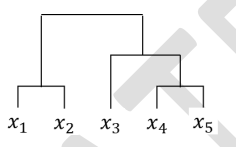
\includegraphics[width=0.22\textwidth]{figs/42a.png} \hfill
    \item 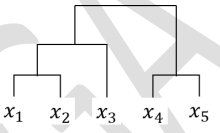
\includegraphics[width=0.22\textwidth]{figs/42b.png} \hfill
    \item 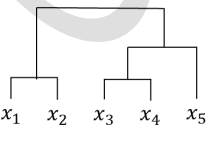
\includegraphics[width=0.22\textwidth]{figs/42c.png} \hfill
    \item 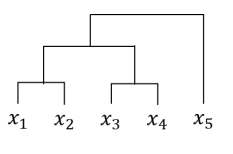
\includegraphics[width=0.22\textwidth]{figs/42d.png}

\qfooter
\end{enumerate} \qfooter
\item Consider the two neural networks (NNs) shown in Fig.~1 and Fig.~2, with $\mathrm{ReLU}$ activation $\mathrm{ReLU}(z) = \max\{0, z\}$. The connections and weights are shown; all biases = 0. For what values of $p, q, r$ in Fig.~2 are the two NNs equivalent when $x_1,x_2,x_3$ are positive?

\begin{figure}[h]
    \centering
    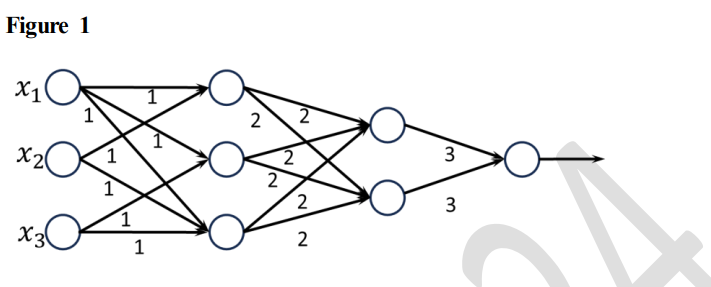
\includegraphics[width=0.45\columnwidth]{figs/q43a.png}
    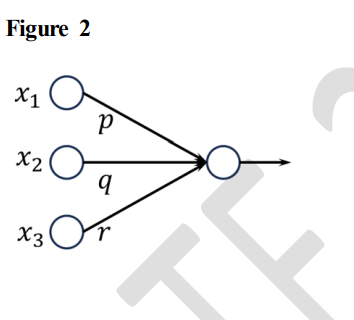
\includegraphics[width=0.45\columnwidth]{figs/q43b.png}
\label{fig:q43a,q43b}
\end{figure}

\begin{enumerate}
\item $p = 36,\ q = 24,\ r = 24$
\item $p = 24,\ q = 24,\ r = 36$
\item $p = 18,\ q = 36,\ r = 24$
\item $p = 36,\ q = 36,\ r = 36$
\qfooter
\end{enumerate} \qfooter

\item Consider a state space where the start state is number 1. The successor function for the state numbered $n$ returns two states numbered $n+1$ and $n+2$. Assume that the states in the unexpanded state list are expanded in the ascending order of numbers and the previously expanded states are not added to the unexpanded state list. Which ONE of the following statements about breadth-first search (BFS) and depth-first search (DFS) is true, when reaching the goal state number 6?
\begin{multicols}{2}
\begin{enumerate}
\item BFS expands more states than DFS.
\item DFS expands more states than BFS.
\item Both BFS and DFS expand equal number of states.
\item Both BFS and DFS do not reach the goal state number 6.
\end{enumerate} \qfooter
\end{multicols}

\item Consider the following sorting algorithms:
(i) Bubble sort
(ii) Insertion sort
(iii) Selection sort\\
Which ONE among the following choices of sorting algorithms sorts the numbers in the array [4, 3, 2, 1, 5] in increasing order after exactly two passes over the array?
\begin{multicols}{2}
\begin{enumerate}
\item (i) only
\item (iii) only
\item (i) and (iii) only
\item (ii) and (iii) only
\end{enumerate} \qfooter
\end{multicols}

\item Given the relational schema $R = (U,V,W,X,Y,Z)$ and the set of functional dependencies: $\{U \to V,\, U \to W,\, WX \to Y,\, WX \to Z,\, V \to X\}$. Which of the following functional dependencies can be derived from the above set?
\begin{multicols}{2}
\begin{enumerate}
\item $VW \to YZ$
\item $WX \to YZ$
\item $VW \to U$
\item $VW \to Y$
\end{enumerate} \qfooter
\end{multicols}

\item Select all choices that are subspaces of $\mathbb{R}^3$.\\
Note: $\mathbb{R}$ denotes the set of real numbers.

\begin{enumerate}
\item $\left\{\vec{x} = \begin{pmatrix}x_1\\x_2\\x_3\end{pmatrix} \in \mathbb{R}^3:\;\vec{x} = \alpha \begin{pmatrix}1\\1\\0\end{pmatrix}+\beta\begin{pmatrix}1\\0\\0\end{pmatrix}, \alpha, \beta\in \mathbb{R}\right\}$
\item $\left\{\vec{x} = \begin{pmatrix}x_1\\x_2\\x_3\end{pmatrix} \in \mathbb{R}^3:\;\vec{x} = \alpha^2 \begin{pmatrix}1\\2\\0\end{pmatrix}+\beta^2\begin{pmatrix}1\\0\\1\end{pmatrix}, \alpha, \beta\in \mathbb{R}\right\}$
\item $\left\{\vec{x} = \begin{pmatrix}x_1\\x_2\\x_3\end{pmatrix} \in \mathbb{R}^3:\;5x_1 + 2x_3 = 0,\, 4x_1-2x_2+3x_3=0\right\}$
\item $\left\{\vec{x} = \begin{pmatrix}x_1\\x_2\\x_3\end{pmatrix} \in \mathbb{R}^3:\;5x_1 + 2x_3 + 4 = 0\right\}$
\end{enumerate}
\qfooter


\item Which of the following statements is/are TRUE?\\
Note: $\mathbb{R}$ denotes the set of real numbers.

\begin{enumerate}
\item There exist $M \in \mathbb{R}^{3\times3}$, $p \in \mathbb{R}^3$, and $q \in \mathbb{R}^3$ such that $M\vec{x}=p$ has a unique solution and $M\vec{x}=q$ has infinite solutions.
\item There exist $M \in \mathbb{R}^{3\times3}$, $p \in \mathbb{R}^3$, and $q \in \mathbb{R}^3$ such that $M\vec{x}=p$ has no solutions and $M\vec{x}=q$ has infinite solutions.
\item There exist $M \in \mathbb{R}^{2\times3}$, $p \in \mathbb{R}^2$, and $q \in \mathbb{R}^2$ such that $M\vec{x}=p$ has a unique solution and $M\vec{x}=q$ has infinite solutions.
\item There exist $M \in \mathbb{R}^{3\times2}$, $p \in \mathbb{R}^3$, and $q \in \mathbb{R}^3$ such that $M\vec{x}=p$ has a unique solution and $M\vec{x}=q$ has no solutions.
\end{enumerate} 
\qfooter

\item Let $\mathbb{R}$ be the set of real numbers, $U$ be a subspace of $\mathbb{R}^3$ and $M \in \mathbb{R}^{3\times 3}$ be the matrix corresponding to the projection onto the subspace $U$. Which of the following statements is/are TRUE?

\begin{enumerate}
\item If $U$ is a $1$-dimensional subspace of $\mathbb{R}^3$, then the null space of $M$ is a $1$-dimensional subspace.
\item If $U$ is a $2$-dimensional subspace of $\mathbb{R}^3$, then the null space of $M$ is a $1$-dimensional subspace.
\item $M^2 = M$
\item $M^3 = M$
\end{enumerate} 
\qfooter


\item Consider the function $f: \mathbb{R} \to \mathbb{R}$, where $\mathbb{R}$ is the set of all real numbers,
\begin{align}
f(x) = \frac{x^4}{4} - \frac{2x^3}{3} - \frac{3x^2}{2} + 1
\end{align}
Which of the following statements is/are TRUE?
\begin{multicols}{2}
\begin{enumerate}
\item $x=0$ is a local maximum of $f$
\item $x=3$ is a local minimum of $f$
\item $x=-1$ is a local maximum of $f$
\item $x=0$ is a local minimum of $f$
\end{enumerate} \qfooter
\end{multicols}


\item Consider the directed acyclic graph (DAG) below:

\begin{figure}[h]
\centering
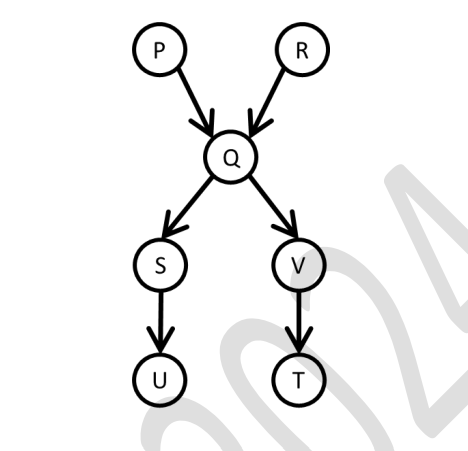
\includegraphics[width=0.55\columnwidth]{figs/51.png}
\label{fig:51}
\end{figure}

Which of the following is/are valid vertex orderings that can be obtained from a topological sort of the DAG?
\begin{enumerate}
\item P Q R S T U V
\item P R Q V S U T
\item P Q R S V U T
\item P R Q S V T U
\qfooter
\end{enumerate} \qfooter
\item Let $H,\,I,\,L,\,N$ represent height, number of internal nodes, number of leaf nodes, and the total number of nodes respectively in a rooted binary tree. Which of the following statements is/are always TRUE?
\begin{multicols}{2}
\begin{enumerate}
\item $L\leq I+1$
\item $H+1 \leq N \leq 2^{H+1}-1$
\item $H\leq I\leq 2^{H}-1$
\item $H\leq L\leq 2^{H}-1$
\end{enumerate} \qfooter
\end{multicols}

% ---------- Q.53 ----------
\item Consider the following figures representing datasets consisting of two-dimensional features with two classes denoted by circles and squares:

\centering
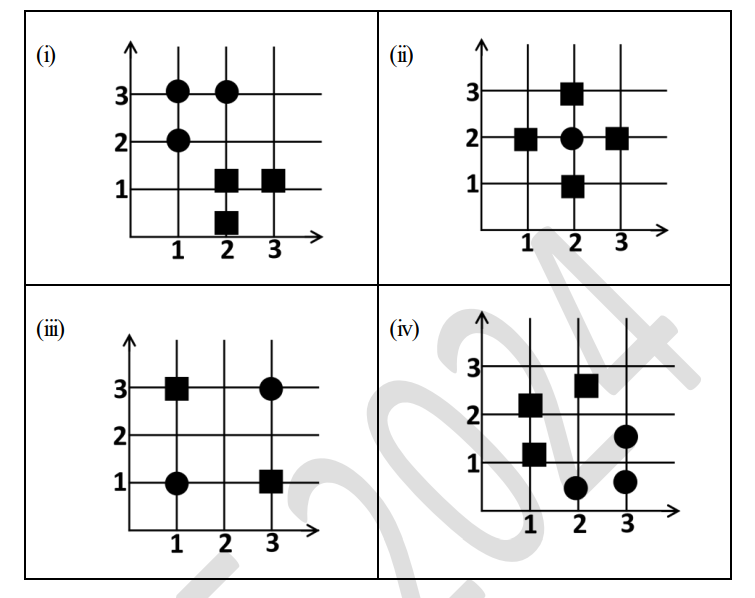
\includegraphics[width=0.85\columnwidth]{figs/53.png}


Which of the following is/are TRUE?
\begin{enumerate}
\item (i) is linearly separable.
\item (ii) is linearly separable.
\item (iii) is linearly separable.
\item (iv) is linearly separable.
\qfooter
\end{enumerate} \qfooter


\item Let \texttt{game(ball, rugby)} be true if the ball is used in rugby and false otherwise. Let \texttt{shape(ball, round)} be true if the ball is round and false otherwise. Consider the following logical sentences:\\
$s_1$: $\forall$ ball $\neg$game(ball, rugby) $\implies$ shape(ball, round)\\
$s_2$: $\forall$ ball $\neg$shape(ball, round) $\implies$ game(ball, rugby)\\
$s_3$: $\forall$ ball $\,\,$game(ball, rugby) $\implies \neg$shape(ball, round)\\
$s_4$: $\forall$ ball $\,\,$shape(ball, round) $\implies \neg$game(ball, rugby)\\
Which of the following choices is/are logical representations of the assertion, ``All balls are round except balls used in rugby''?
\begin{multicols}{2}
\begin{enumerate}
\item $s_1 \wedge s_3$
\item $s_1 \wedge s_2$
\item $s_2 \wedge s_3$
\item $s_3 \wedge s_4$
\end{enumerate} \qfooter
\end{multicols}

\item An OTT company is maintaining a large disk-based relational database of different movies with the following schema:\\
Movie(ID, CustomerRating)\\
Genre(ID, Name)\\
Movie\_Genre(MovieID, GenreID)\\
Consider the following SQL query on the relational database above:
\begin{lstlisting}[language=SQL]
SELECT *
FROM Movie, Genre, Movie_Genre
WHERE Movie.CustomerRating > 3.4
  AND Genre.Name = "Comedy"
  AND Movie_Genre.MovieID = Movie.ID
  AND Movie_Genre.GenreID = Genre.ID;
\end{lstlisting}
This SQL query can be sped up using which of the following indexing options?
\begin{enumerate}
\item B+ tree on all the attributes.
\item Hash index on Genre.Name and B+ tree on the remaining attributes.
\item Hash index on Movie.CustomerRating and B+ tree on the remaining attributes.
\item Hash index on all the attributes.
\end{enumerate} 
\qfooter


\item Let $X$ be a random variable uniformly distributed in the interval $[1, 3]$ and $Y$ be a random variable uniformly distributed in the interval $[2, 4]$. If $X$ and $Y$ are independent of each other, the probability $P(X\geq Y)$ is \rule{7em}{0.07em} (rounded off to three decimal places).
\qfooter

\item Let $X$ be a random variable exponentially distributed with parameter $\lambda > 0$. The probability density function of $X$ is given by:\\
$f_X(x) = \begin{cases} \lambda e^{-\lambda x}, & x\geq 0\\ 0, & \text{otherwise} \end{cases}$\\
If $5E(X) = Var(X)$, where $E(X)$ and $Var(X)$ indicate the expectation and variance of $X$, respectively, the value of $\lambda$ is \rule{7em}{0.07em} (rounded off to one decimal place).
\qfooter

\item Consider two events $T$ and $S$. Let $\bar{T}$ denote the complement of the event $T$. The probability associated with different events are given as follows:\\
$P(\bar{T}) = 0.6$, $P(S|T) = 0.3$, $P(S|\bar{T}) = 0.6$\\
Then, $P(T|S)$ is \rule{6em}{0.07em} (rounded off to two decimal places).
\qfooter

\item Consider a joint probability density function of two random variables $X$ and $Y$:
\begin{align}
f_{X,Y}(x, y) = \begin{cases}
2xy,& 0 < x < 2,\ 0 < y < x\\
0,& \text{otherwise}
\end{cases}
\end{align}
Then, $E[Y|X=1.5]$ is \rule{7em}{0.07em}.
\qfooter

\item Evaluate the following limit:
$\displaystyle \lim_{x\to 0} \frac{\ln((x^2+1)\cos x)}{x^2} = \rule{7em}{0.07em}$
\qfooter



\item Let $\vec{u} = [1\ 2\ 3\ 4\ 5]^T$, and let $\sigma_1, \sigma_2, \sigma_3, \sigma_4, \sigma_5$ be the singular values of the matrix $M = \vec{u} \vec{u}^T$ (where $\vec{u}^T$ is the transpose of $\vec{u}$). The value of $\sum\limits_{i=1}^{5} \sigma_i$ is \rule{7em}{0.07em}.
\qfooter

% ---------- Q.62 ----------
\item Details of ten international cricket games between two teams “Green” and “Blue” are given in Table~C. 
This table lists matches played on different pitches, across formats, along with their winners.  
Pitch can be spin-friendly (S) or pace-friendly (F).  
Format can be one-day (O) or test (T).

A cricket organization would like to use this data to develop a decision-tree model to predict outcomes.  
The computed $\mathrm{InformationGain}(\mathrm{C}, \mathrm{Pitch})$ with respect to the Target is \rule{2cm}{0.15mm} (rounded off to two decimal places).
\begin{table}[h]
\centering
\begin{tabular}{|c|c|c|c|}
\hline
Match No. & Pitch & Format & Winner (Target) \\
\hline
1 & S & T & Green \\
2 & S & T & Blue \\
3 & F & O & Blue \\
4 & S & O & Blue \\
5 & F & T & Green \\
6 & F & O & Blue \\
7 & S & O & Green \\
8 & F & T & Blue \\
9 & F & O & Blue \\
10 & S & O & Green \\
\hline
\end{tabular}
\end{table}
\qfooter

\qfooter

% ---------- Q.63 ----------
\item Given the two-dimensional dataset consisting of 5 data points from two classes (circles and squares)  
and using Euclidean distance as the metric, the minimum odd value of $k$ in the $k$-nearest neighbour algorithm  
for which the diamond ($\lozenge$) point is assigned the label ``square'' is \rule{2cm}{0.15mm}.

\begin{figure}[H]
\centering
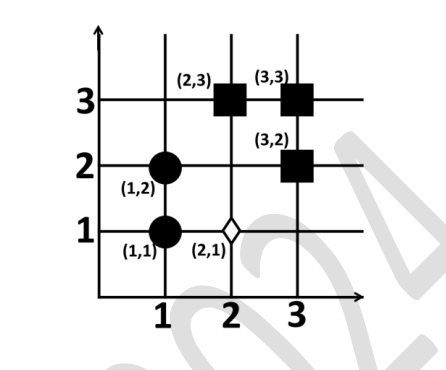
\includegraphics[width=0.45\columnwidth]{figs/63.png} % replace with actual KNN dataset figure
\label{fig:63}
\end{figure}
\qfooter


% ---------- Q.64 ----------
\item Given the following Bayesian Network of four Bernoulli random variables and the associated conditional probability tables:

\begin{center}
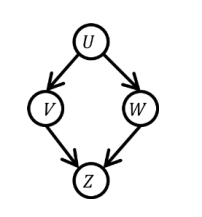
\includegraphics[width=0.75\columnwidth]{figs/64.png} % replace with actual Bayesian network figure
\end{center}

The value of $P(U=1, V=1, W=1, Z=1)$ is \rule{1cm}{0.075mm} (rounded off to three decimal places).
\qfooter


\item Two fair coins are tossed independently. $X$ is a random variable that takes a value of $1$ if both tosses are heads and $0$ otherwise. $Y$ is a random variable that takes a value of $1$ if at least one of the tosses is heads and $0$ otherwise. The value of the covariance of $X$ and $Y$ is \rule{7em}{0.07em} (rounded off to three decimal places).

\end{enumerate} 
\qfooter

\end{document}
